
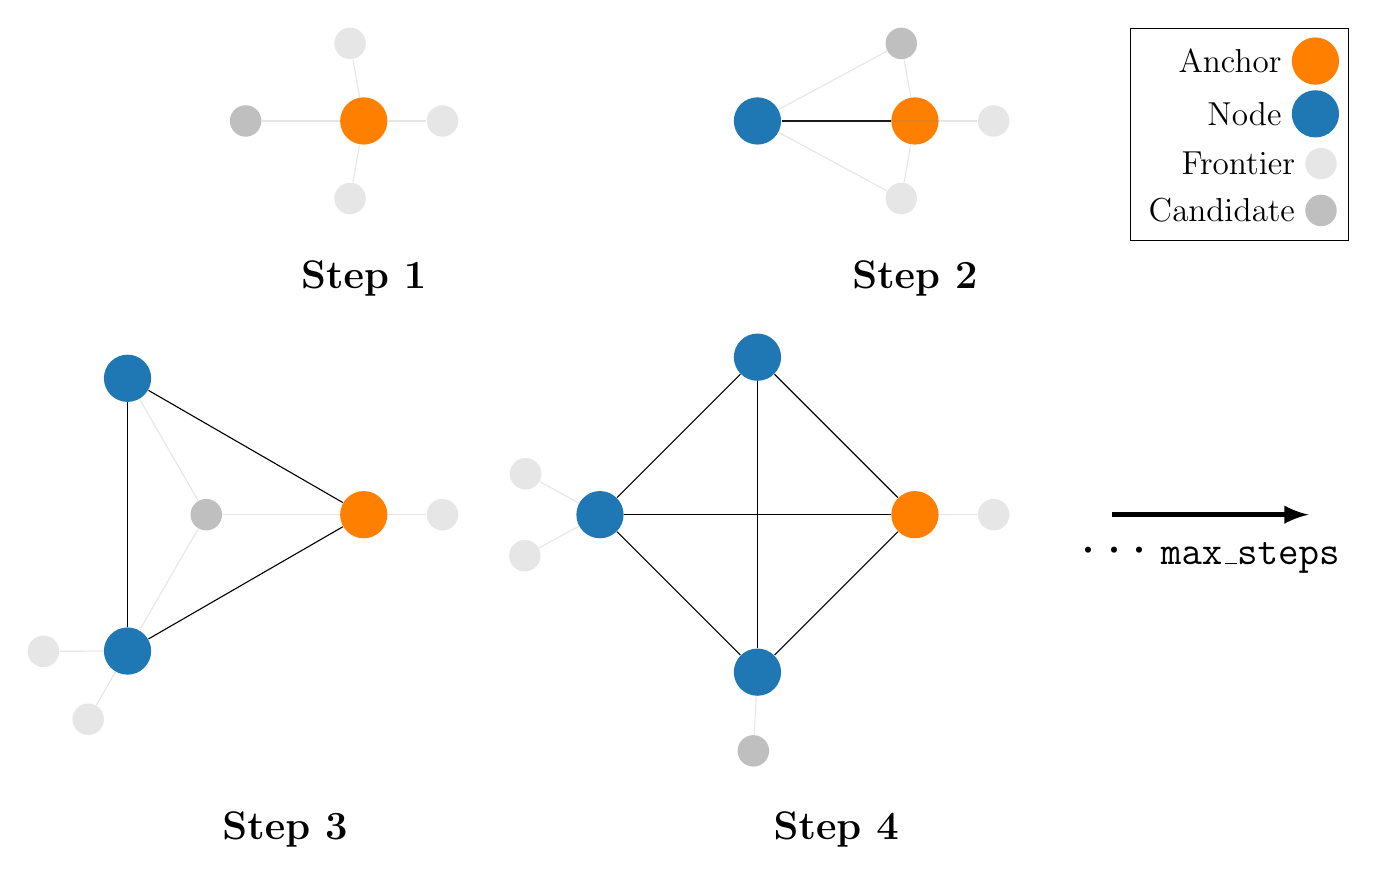
\begin{tikzpicture}[
  scale=1,   
  anchornode/.style={fill=orange, minimum size=6mm, circle},
  frontiernode/.style={fill=gray, minimum size=4mm, circle, opacity=0.2},
  nodenode/.style={fill={rgb,255:red,31;green,119;blue,180}, minimum size=6mm, circle},
  candidatenode/.style={fill=gray, minimum size=4mm, circle, opacity=0.5}
]
  % \Large \textbf{Step} 1
  \begin{scope}[shift={(2,0)}]
    \draw
      (0.0:0) node[anchornode] (0){}
      (0.0:1) node[frontiernode] (-1){}
      (0.0:-1.5) node[candidatenode] (-2){}
      (100:1) node[frontiernode] (-3){}
      (260:1) node[frontiernode] (-4){};
    \begin{scope}[-]
      \draw[draw=gray, thin, opacity=0.2] (0) to (-1);
      \draw[draw=gray, thin, opacity=0.2] (0) to (-2);
      \draw[draw=gray, thin, opacity=0.2] (0) to (-3);
      \draw[draw=gray, thin, opacity=0.2] (0) to (-4);
    \end{scope}
    \node at (0,-2) {\Large \textbf{Step 1}};
  \end{scope}

  % \Large \textbf{Step} 2
  \begin{scope}[shift={(9,0)}]
    \draw
      (0.0:0) node[anchornode] (0){}
      (0.0:1) node[frontiernode] (-1){}
      (180.0:2) node[nodenode] (1){}
      (100:1) node[candidatenode] (-3){}
      (260:1) node[frontiernode] (-4){};
    \begin{scope}[-]
      \draw (0) to (1);
      \draw[draw=gray, thin, opacity=0.2] (0) to (-3);
      \draw[draw=gray, thin, opacity=0.2] (1) to (-1);
      \draw[draw=gray, thin, opacity=0.2] (-3) to (1);
      \draw[draw=gray, thin, opacity=0.2] (0) to (-4);
      \draw[draw=gray, thin, opacity=0.2] (1) to (-4);
    \end{scope}
    \node at (0,-2) {\Large \textbf{Step 2}};
  \end{scope}

  % \Large \textbf{Step} 3
  \begin{scope}[shift={(0,-5)}]
    \draw
      (0.0:0) node[fill=gray, minimum size=4mm, circle, opacity=0.5] (-6){}
      (0.0:3) node[frontiernode] (-1){}
      (0.0:2) node[anchornode] (0){}
      (120.0:2) node[nodenode] (1){}
      (240.0:3) node[frontiernode] (-4){}
      (220.0:2.7) node[frontiernode] (-5){}
      (240.0:2) node[nodenode] (2){};
    \begin{scope}[-]
      \draw[draw=gray, thin, opacity=0.2] (0) to (-1);
      \draw (0) to (1);
      \draw (0) to (2);
      \draw (1) to (2);
      \draw[draw=gray, thin, opacity=0.2] (2) to (-4);
      \draw[draw=gray, thin, opacity=0.2] (2) to (-5);
      \draw[draw=gray, thin, opacity=0.2] (1) to (-6);
      \draw[draw=gray, thin, opacity=0.2] (2) to (-6);
      \draw[draw=gray, thin, opacity=0.2] (0) to (-6);
    \end{scope}
    \node at (1,-4) {\Large \textbf{Step 3}};
  \end{scope}

  % \Large \textbf{Step} 4
  \begin{scope}[shift={(7,-5)}]
    \draw
      (0.0:3) node[frontiernode] (-1){}
      (0.0:2) node[anchornode] (0){}
      (90.0:2) node[nodenode] (1){}
      (180.0:2) node[nodenode] (2){}
      (270.0:2) node[nodenode] (3){}
      (269.0:3) node[candidatenode] (-6){}
      (190.0:3) node[frontiernode] (-4){}
      (170.0:2.99) node[frontiernode] (-5){};
    \begin{scope}[-]
      \draw[draw=gray, thin, opacity=0.2] (0) to (-1);
      \draw (0) to (1);
      \draw (0) to (2);
      \draw (0) to (3);
      \draw (1) to (2);
      \draw (1) to (3);
      \draw (2) to (3);
      \draw[draw=gray, thin, opacity=0.2] (2) to (-4);
      \draw[draw=gray, thin, opacity=0.2] (2) to (-5);
      \draw[draw=gray, thin, opacity=0.2] (3) to (-6);
    \end{scope}
    \node at (1,-4) {\Large \textbf{Step 4}};
  \end{scope}

  % Dots
  \begin{scope}[shift={(11,-8)}]
    \draw[->, >=latex, line width=2pt] (0.5,3) --  node[label= below:\Large\textbf{\huge $\cdots$} \texttt{max\_steps}] {} (3,3);
  \end{scope}

  \matrix [draw, below left, row sep=2pt] at (current bounding box.north east) {
    \node [anchornode, label=left:{\large Anchor}] {}; \\ 
    \node [nodenode, label=left:{\large Node}] {}; \\
    \node [frontiernode, label=left:{\large Frontier}] {}; \\
    \node [candidatenode, label=left:{\large Candidate}] {}; \\
  };
\end{tikzpicture}
